\section{Part I}\label{P1}

\subsection{8-point algorithm function (version 1)}

In order to implement this algorithm, it is essential to initially construct the "A" matrix for the linear homogeneous system. To accomplish this, the \texttt{EightPointsAlgorithm(P1, P2)} function is invoked with the corresponding points $P1$ and $P2$. Subsequently, the Singular Value Decomposition ($\text{SVD}(A) = [U \ D \ V]$) is employed to produce the unit matrix $V$ and to identify the final column of $V$ as the solution, which is a $9 \times 1$ vector. For the $F$ matrix to be constructed, the subsequent step is to restructure the $9 \times 1$ matrix into a $3 \times 3$ matrix using \texttt{reshape( , [3 3])}. The matrix $F$ must have rank 2, and we manually achieve this. Using the $\text{SVD}(F) = [U \ D \ V]$, we then set $D[3,3]$ of the matrix $D$ to 0. The $F$ matrix is subsequently recomputed using $U D V^T$, in which $D[3,3]$ is equal to zero.

\subsection{8-point algorithm function (version2)}

The normalized eight-point algorithm is employed to improve the accuracy of the fundamental matrix estimation. Initially, the input points are normalized, and the eight-point algorithm from the final section is implemented. The previous algorithm's stages will be executed once more on the normalized corresponding points in the \texttt{EightPointsAlgorithmN(P1, P2)}. In order to emphasize the point, $P1$ and $P2$ must be normalized using the \texttt{normalise2dpts(P1)} function. Subsequently, the new $F$ is generated by denormalizing the functionality matrix $F$ using the \texttt{EightPointsAlgorithm(P1, P2)}. 

It is imperative to emphasize that all of the points are presented in a uniform manner. The numerical stability of the solution can be enhanced by normalizing the input points, which is involved in the solution of a linear system of equations in the 8-point algorithm. It aids in the prevention of problems associated with ill-conditioned matrices that may occur when dealing with large or small numbers in the input data. The algorithm becomes less susceptible to anomalies and noise in the data by establishing a common scale for the point coordinates. The fundamental matrix is defined to scale. The algorithm's scale-invariance is guaranteed by normalizing the coordinates. Normalization facilitates the optimization process by facilitating the attainment of more dependable and expedited convergence. It can enhance the solution's robustness, particularly in situations where the point correspondences exhibit a broad spectrum of scales.


\begin{figure} [ht]
    \centering
    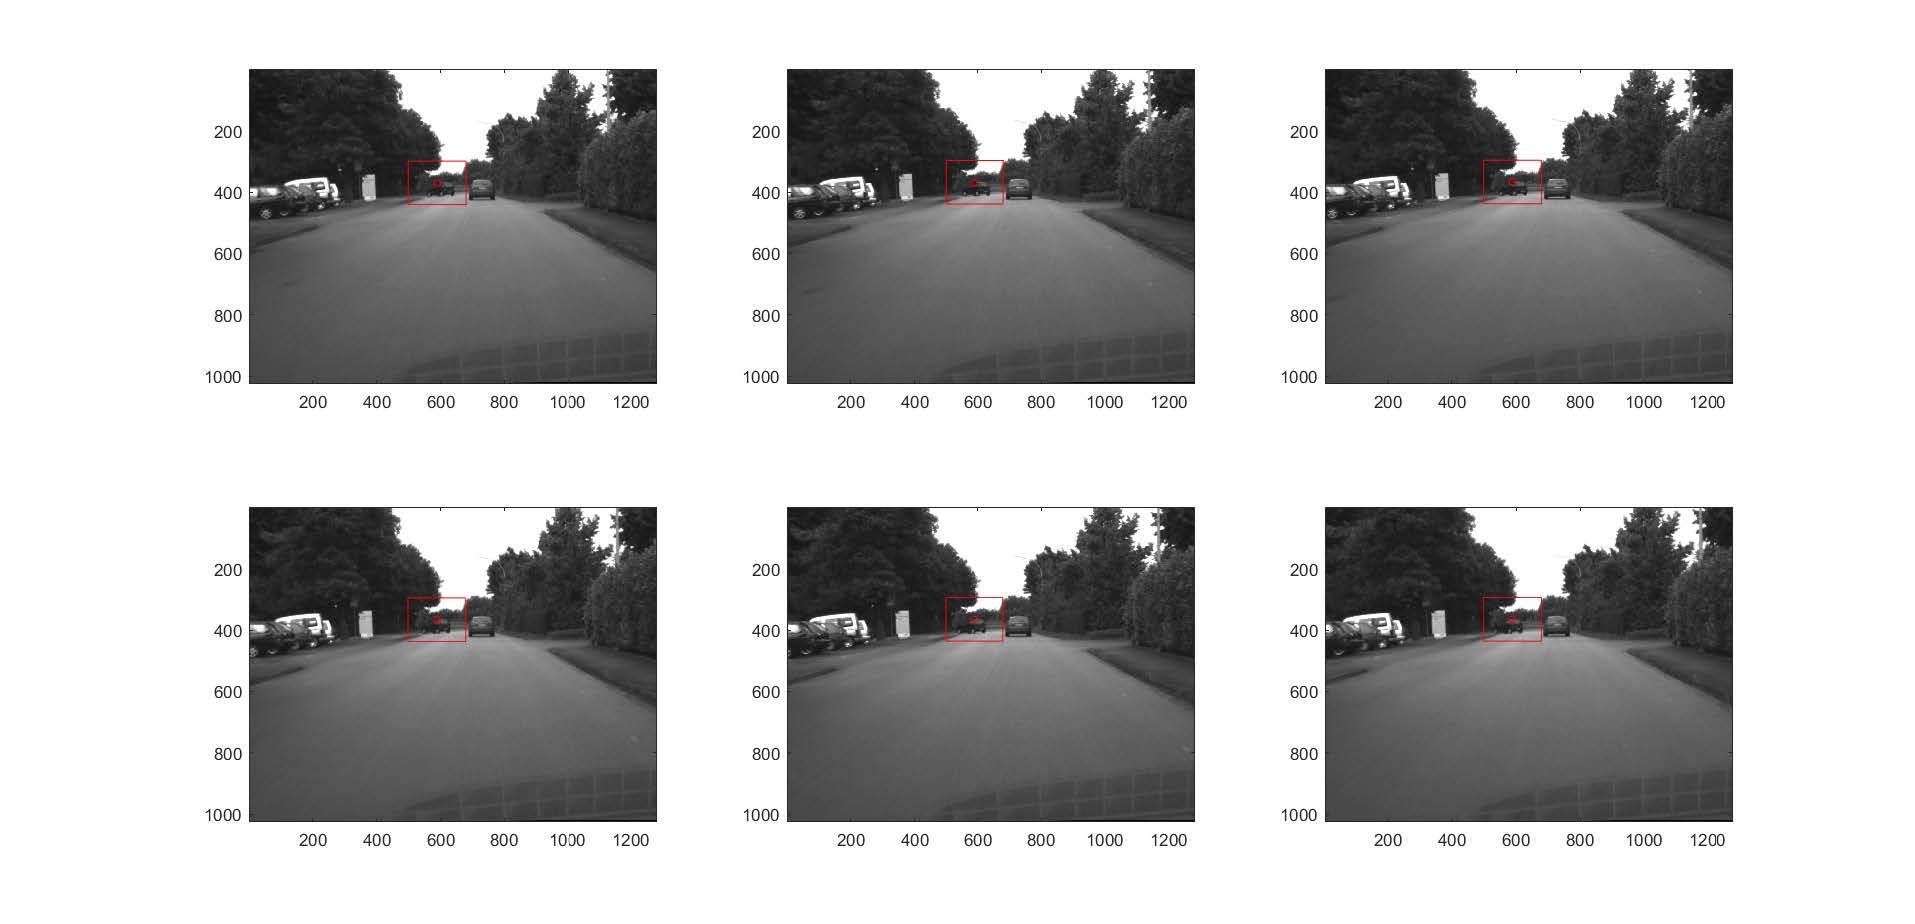
\includegraphics[width = 0.9\textwidth]{Resources/F8-1.jpg}
    \caption{The Second results of detecting objects with larger frames}
    \label{fig:The Second results of detecting objects with larger frames}
\end{figure}